%-%-%-%-%-%-%-%-%-%-%-%-%-%-%-%-%-%-%-%-%-%-%-%-%-%
% EE531: laboratório de Eletrônica Básica I       %  
% Experimento 2: Diodos                           %
% Data:20/08/2010                                 %
% Unicamp,Campinas,São Paulo,Brasil               % 
% Grupo:                                          %
%       - Daniel Lins Mattos                      %
%       - Raquel Mayumi Kawamoto                  %
%       - Tiago Chedraoui Silva                   % 
%-%-%-%-%-%-%-%-%-%-%-%-%-%-%-%-%-%-%-%-%-%-%-%-%-%
%\documentclass[letter]{article}  % formato impressao IC
\documentclass[a4paper]{article} % formato impressao FEEC

%%% fontes %%%
\usepackage[T1]{fontenc}
\usepackage[brazil]{babel}    % dá suporte para os termos na língua portuguesa do Brasi
\usepackage[utf8]{inputenc}   % acentuação
\usepackage{ae,aecompl,aeguill}       % pdfs mais bonitos =)

%%% outros %%%
\usepackage{multirow}
\usepackage{textcomp}
\usepackage{color}       
\usepackage{indentfirst}      % retira padrao americano de paragrafos
\usepackage{multicol}   
\usepackage[linkbordercolor={1 1 1},urlcolor=black,colorlinks=true]{hyperref} % links
\usepackage{subfig}
\usepackage[letterpaper]{geometry}
\geometry{verbose,lmargin=3cm,rmargin=3cm}

% circuito eletrico
\usepackage{electComp}
\usetikzlibrary{decorations,decorations.pathmorphing,decorations.pathreplacing}
\usepackage{verbatim}
\usepackage{pstricks}
\usepackage{boxdims}

\setcounter{tocdepth}{0}
\renewcommand{\thefigure}{\thesubsection.\arabic{figure}}
\date{Setembro 10, 2010}
% Capa estilizada %
\newcommand*{\titleTMB}{\begingroup \centering \settowidth{\unitlength}{\LARGE EE531} {\large\scshape EE531 - Turma S}\\[0.2\baselineskip] \rule{11.0cm}{1.6pt}\vspace*{-\baselineskip}\vspace*{2pt} \rule{11.0cm}{0.4pt}\\[\baselineskip] {\LARGE  Diodos}\\\vspace*{\baselineskip}  {\itshape Laboratório de Eletrônica Básica I - Segundo Semestre de 2010}\\ \rule{11.0cm}{0.4pt}\vspace*{-\baselineskip}\vspace{3.2pt} \rule{11.0cm}{1.6pt}\\[\baselineskip] {\large\scshape Professor: José Cândido Silveira Santos Filho}\par \vfill {\normalsize   \scshape 
    \begin{center} 
      \begin{tabular}{  l  l  p{5cm} } 
 	Daniel Lins Mattos & RA: 059915\\
        Raquel Mayumi Kawamoto & RA: 086003\\
        Tiago Chedraoui Silva  & RA: 082941\\
      \end{tabular} \end{center}
    \itshape 10 de setembro de 2010    }\\[\baselineskip] \vspace{3.2pt} \endgroup}


\begin{document}
\titleTMB 
\newpage


Este experimento visa o estudo do diodo semicondutor, elemento não-linear
fundamental de um circuito. Assim como um resistor, o diodo tem dois terminais; mas,diferentemente do resistor, o qual tem uma relação linear (direta) entre a corrente que circula por ele e a tensão aplicada, o diodo tem uma característica i-v não-linear.
      Portanto, para um melhor entendimento do funcionamento e das características de um diodo, este experimento trata da aplicação mais comum do diodo, o projeto de circuitos retificadores (o qual converte ca em cc).

        Assim como no primeiro experimento, foi utilizado o protoboard para a montagem dos
circuitos. Foi necessário, ainda, a utilização de oito diodos 1N4001 ou 1N4002, dois diodos
1N4148, três capacitores eletrolíticos $100\mu$F,  um amplificador operacional 741, dois resistores
de $10k\Omega$, um resistor de $1k\Omega$ e um tranformador de 110 $V_{ac}$,9 $V_{ac}$.


\section*{Parte Experimental}
%\begin{enumerate}
%\item
\section{Amplificador Operacional}
 \setcounter{figure}{0}
Um amplificador operacional é um amplificador com ganho  muito elevado. Tem dois terminais de entrada: um terminal designado por terminal inversor(-) e o outro identificado por terminal não inversor(+).
Um amplificador operacional ideal possui algumas características como ter um ganho infinito em malha aberta, impedância de entrada infinita e impedância de saída nula. 

 Para esta parte inicial do experimento, o circuito da figura \ref{circ:1} --- composto de um amplificador operacional 741, um resistor (R$_i$) de $1k\Omega$, e dois diodos 1n4148 (D$_1$ e D$_2$) --- é montado e o canal um do osciloscópio é colocado entre D$_1$ e R$_i$ e o canal dois na saída do amplificador operacional. 

Além disso, o gerador de funções é ajustado para produzir um sinal de tensão com sua forma de onda triangular, com amplitude 10$V_{pp}$, com offset de $5V$, frequência de $10kHz$ e simetria de 50\%. 

 É importante que a onda gerada seja positiva, pois caso fosse negativa diodo $D_1$ atuaria bloquearia o sinal, logo o amplificador operacional saturaria.

\vspace{3mm}
\begin{figure}[h]
\centerline{\input circ1.tex}
\caption{Circuito para caracterização V versus I do diodo \label{circ:1}}
\end{figure}

Supondo que o amplificador operacional seja ideal, nenhuma corrente de entrada é drenada, ou seja, a corrente $i$ caracterizada em $D_1$ e $R_i$ é a mesma que em $D_2$. Além disso, a tensão entre o terminal de saída e o terra é equivalente a $A(v_2-v_1)$, sendo o ganho $A$ idealmente infinito. Logo, tem-se que:
\begin{equation}
\frac{V_D}{A}=(v_2-v_1)\approx0
\end{equation}

Como $v_1=0$ temos que $v_2=0$, assim:.
\begin{equation}
i=\frac{V_{CH2}}{R_{i}}\\
\end{equation}

Utilizando o canal 1, tem-se que:  
\begin{equation}
V_D=-V_{CH1}\\
\end{equation}

\newpage
Utilizando o recurso Time Base X-Y do osciloscópio, obtemos uma curva caracterísica (V versus I) do diodo presente na figura \ref{fig:q1-curva2}. As escala do eixo $V_D$ vale $500mV$/célula. Portanto, o diodo em condução direta apresenta um queda de tensão de aproximadamente $0,7V$.    
\begin{figure}[h]
\begin{centering}
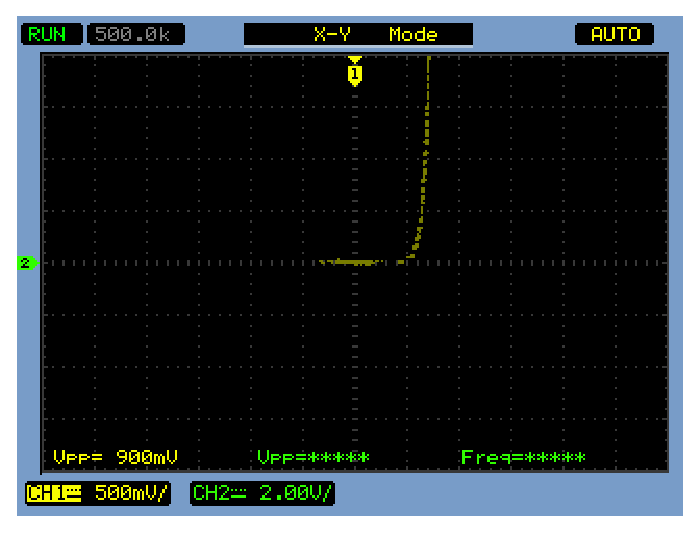
\includegraphics[scale=0.7]{Imagens/3.1/NewFile0} \caption{Curva característica V versus I do diodo  \label{fig:q1-curva2}}
\par\end{centering}
\end{figure}

\begin{figure}[h]
\begin{centering}
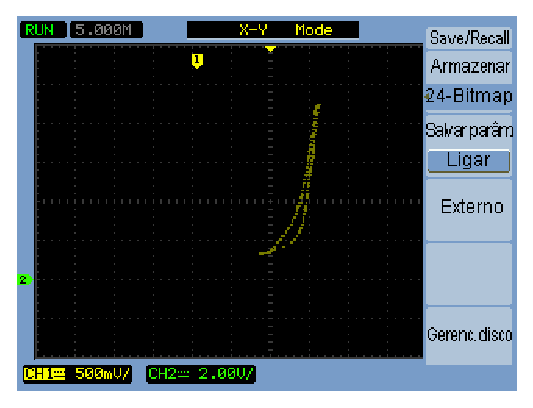
\includegraphics[scale=1.0]{Imagens/3.1.opcional/opcio} \caption{Curva de histerese \label{fig:q1-his}}
\par\end{centering}
\end{figure}


\newpage
\section{Circuitos retificadores}
 \setcounter{figure}{0}
O circuito retificador é uma aplicação fundamental do diodo, que faz uso intenso da curva não-linear i-v. Este circuito consiste em um diodo D e um resistor R conectados em série.Supondo uma tensão de entrada senoidal  $v_1$ e um diodo ideal, durante os semicilos positivosda entrada senoidal, a tensão positiva  $v_1$     faz com que a corrente circule pelo diodo no sentido
direto. Como a tensão no diodo será muito pequena, idealmente zero, a tensão de saída  $v_0$ será igual a tensão de entrada      $v_1$     . Durante os semiciclos negativos de    $v_1$    , o diodo não conduzirá. Portanto,   $v_0$     será zero. A figura 2.1 ilustra os circuitos em cada semiciclo de   $v_1$  e as formas de ondas de saída  $v_0$      .
        Observa-se que, enquanto  $v_1$        alterna em polaridade e tem um valor médio zero,     $v_0$   é unidirecional e tem um valor médio finito, ou uma componente cc. Portanto, o circuito retificador retifica o sinal, sendo por isso denominado de retificador. Ele pode ser usado para gerar cc a partir de ca.
         Para este experimento foram estudados dois tipos de circuitos retificadores: retificador
de meia onda e retificador de onda completa tipo ponte.
      
\subsection{Retificador de meia onda}
         Inicialmente foi montado no protoboard o circuito da figura 2.1.1 circuito retificador de meia onda que consiste em um diodo de retificação (diodo 1N4001) e um resistor (de valor $10k\Omega$) conectados em série, alimentados por um transformador de $110V_{ac}$.
         Um circuito retificador de meia onda utiliza metade dos semiciclos da senóide de entrada. Supondo um diodo ideal, durante os semiciclos positivos da entrada senoidal, a tensão positiva $V_s$ faz com que a corrente circule pelo diodo no sentido direto. Segue que a tensão no diodo será muito pequena idealmente zero. Portanto, a tensão de saída $V_0$ será igual à tensão de entrada $V_s$ . Por outro lado, durante os semiciclos negativos de $V_s$, o diodo não conduzirá, sendo a tensão de saída igual a zero. Enquanto $V_s$ alterna em polaridade e tem um valor médio zero, a tensão de saída é unidirecional e tem um valor médio finito, ou uma componente cc.
         Como o diodo do circuito da figura 2.1.1 não é ideal, pode-se escrever:
     
\begin{equation}
v_0=0,  v_s<V_{DO}
\end{equation}
\begin{equation}
v_0=\frac{R}{R+r_D}v_s -V_{DO}\frac{R}{R+r_D},  v_s>=V_{DO}
\end{equation}


    Em que   $V_{DO}$     e $r_D$ são, respectivamente, a tensão e a resistência do diodo.
         Em muitas aplicações tem-se  $r_D << R$           e a segunda equação pode ser simplificada para:
\begin{equation}
v_0=v_s-V_{DO}
\end{equation}


         Um dos principais parâmetros de um diodo no projeto de retificadores é a tensão de pico inversa (\textit{peak inverse voltage} – PIV) que o diodo deve ser capaz de suportar sem atingir a
tensão de ruptura, determinada pelo maior valor de tensão inversa que pode aparecer no diodo. Pelo circuito da figura  \ref{fig:ret-circ1} observa-se que, quando $v_s$ é negativo, o diodo corta e   $v_0$      é
igual a zero. Portanto, conclui-se que a PIV é igual ao valor de pico $v_s:PIV=V_s$ .

\begin{figure}[h!]
\begin{centering}
\subfloat[]{
%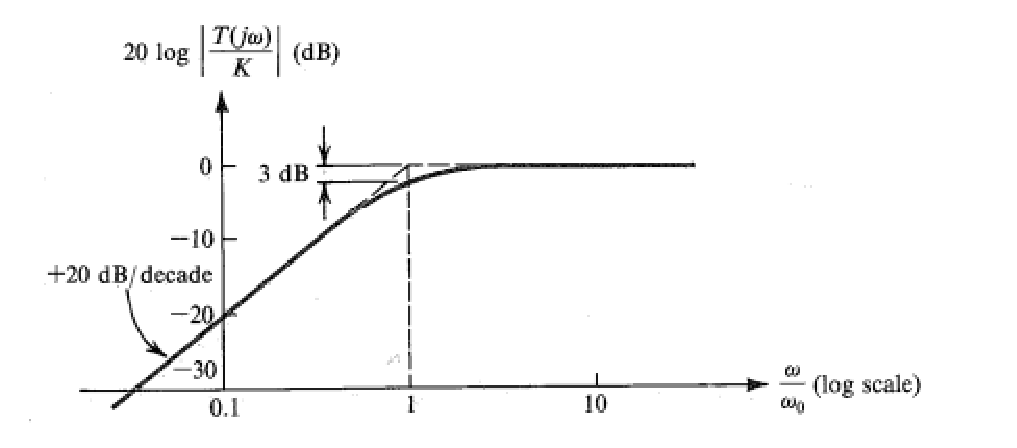
\includegraphics[scale=0.45]{Imagens/mag_h.eps}
\input circ2.tex
 \label{fig:ret-circ1(a)}
}

\subfloat[]{
\includegraphics[scale=0.7]{Imagens/3.3.1ret_meia_onda/311}
 \label{fig:ret-circ1(b)}
}
\par\end{centering}
\caption{(a) Circuito Retificador de Meia Onda. (b)  Formas de onda de entrada e saída. \label{fig:ret-circ1}}
\end{figure}

\newpage
          Fazendo-se a análise do esquemático da figura  \ref{fig:ret-circ1(a)}, pode-se ver o funcionamento de um retificador de meia onda a partir das formas de ondas capturadas no osciloscópio dos nós 1 e 2 do circuito da figura  \ref{fig:ret-circ1(b)}. Os nós 1 e 2 correspondem, respectivamente, ao canal 1(CH1) e ao canal 2 (CH2) do osciloscópio. Nos semiciclos positivos, como o diodo encontra-se em curto, irá passar corrente pelo circuito, criando uma tensão de saída no resistor. Os diodos introduzem perdas na tensão final de modo que a tensão de saída tende a $v_0=v_s-V_{DO}$.Pode-se verificar pela figura  \ref{fig:ret-circ1(b)} que a máxima tensão de saída do circuito é de   $13.4 Volts$. Portanto,    $V_{DO}= 0.8V $ . Nos semiciclos negativos, o diodo não conduz, portanto a tensão de saída é zero.
    


 \subsection{ Retificador de Onda Completa tipo Ponte}
         Foi montado no protoboard o circuito da figura 2.2.1 circuito retificador de onda completa tipo ponte que consiste em quatro diodos de retificação $D$ (diodo 1N4001) e um resistor $R$    (de valor $10k\Omega$) dispostos conforme indica a figura 2.2.1, alimentados por um transformador de $110V_{ac}$.
         O circuito retificador em ponte opera da seguinte maneira: durante os semiciclos positivos da tensão de entrada $v_s$, é positiva e a corrente é conduzida pelo diodo $D_1$, resistor $R$ e diodo $D_2$. Enquanto isso, os diodos  $D_3$      e $D_4$   estarão inversamente polarizados. Durante os semiciclos negativos da tensão de entrada, a tensão $v_s$ no secundário será negativa e, portanto,  $-v_s$     será positiva, forçando a corrente a circular por $D_3$ , $R$ e $D_4$ . Enquanto isso, os diodos $D_1$ e $D_2$   estarão inversamente polarizados.
         Deve ser observado que durante ambos os semiciclos, a corrente circula por $R$ no mesmo sentido (do ponto 3 para o ponto 0) e então   $v_o$    será sempre positiva.
         Para determinar a tensão de pico inversa (PIV) de cada diodo, considera-se o circuito durante os semiciclos positivos. A tensão inversa sobre o diodo $D_3$ pode ser estabelecida pela malha formada por $D_3$, R e $D_2$         como  $v_{D3}(inverso)v_o+v_{D2}(direto)$ . Logo, o valor máximo de $v_{D3}$     ocorre no pico de $v_o$    e é dado por:
                                    
\begin{equation}
PIV=V_S-2V_D+V_D=V_S-V_D
\end{equation}

%\newpage
\begin{figure}[h!]
\begin{centering}
\subfloat[]{
%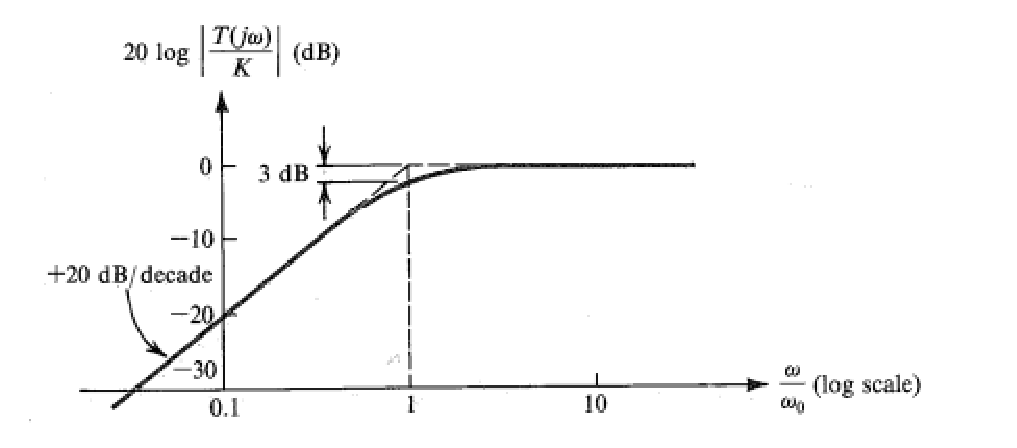
\includegraphics[scale=0.45]{Imagens/mag_h.eps}
\input circ3.tex
 \label{fig:ret-circ2(a)}
}
\par\end{centering}
\subfloat[]{
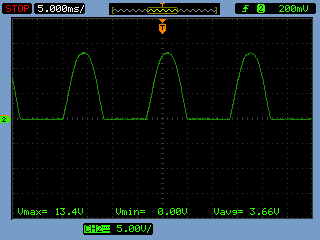
\includegraphics[scale=0.45]{Imagens/3.3.1onda_completa/p2q3}
 \label{fig:ret-circ2(b)}
}
\subfloat[]{
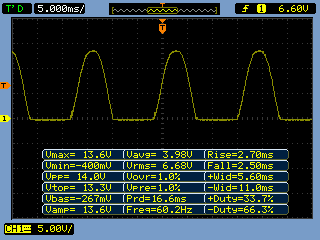
\includegraphics[scale=0.45]{Imagens/3.3.1onda_completa/no2}
\label{fig:ret-circ2(c)}
}
\subfloat[]{
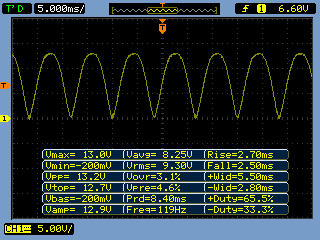
\includegraphics[scale=0.45]{Imagens/3.3.1onda_completa/no3}
\label{fig:ret-circ2(d)}
}

\caption{(a) Circuito Retificador de Onda Completa tipo Ponte. (b) Forma de onda
no ponto do nó 1. (c) Forma de onda no ponto do nó 2. (d) Forma de onda no ponto do nó 3. \label{fig:ret-circ2}}
\end{figure}


    Com o objetivo de montar uma fonte de tensão DC não regulada, introduziu-se o capacitor eletrolítico de  $100\mu$F entre os nós 3 e 0 da Figura \label{fig:ret-circ2}, ou seja, o capacitor é incluído em paralelo com o resistor de carga. Dessa forma, obteve-se um circuito retificador com capacitor de filtro (o retificador de pico).
         O circuito retificador de pico opera da seguinte maneira: inicialmente, o capacitor está descarregado; durante o primeiro semiciclo da tensao do secundário, o diodo está conduzindo permitindo que o secundário carregue o capacitor até a tensão de pico; logo após, no semiciclo negativo, o diodo pára de conduzir (o que significa uma chave aberta) e neste estágio, como o capacitor tem uma tensão $V_p$, ele polariza o diodo inversamente e começa a descarregar-se no resistor de carga. Deve ser considerado a constante de tempo de descarga do capaciotr, que é função do resistor $R$ e do capacitor $C$. Esta constante deve ser bem maior do que o período $T$ do sinal de entrada. Dessa forma, o capacitor só se descarregará um pouco até o próximo ciclo.

A figura \ref{fig:cap-ret} ilustra a forma de onda do retificador de pico.
  %  Figura 2.2.2 

\begin{figure}[h!]
\begin{centering}
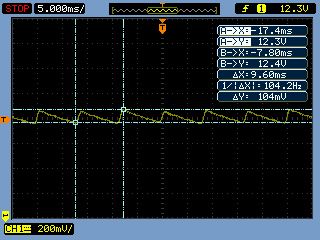
\includegraphics[scale=0.7]{Imagens/3.3.4capacitor_paralelo/3cap} \caption{Forma de onda da tensão no capacitor do retificador de pico. \label{fig:cap-ret}}
\par\end{centering}
\end{figure}

\newpage
\section{Duplicador de Tensão}
 \setcounter{figure}{0}
\vspace{3mm}
\begin{figure}[h]
\centerline{\input circ4.tex}
\caption{Duplicador de tensão \label{tab:circ}}
\end{figure}


\newpage
\begin{figure}[h!]
\begin{centering}
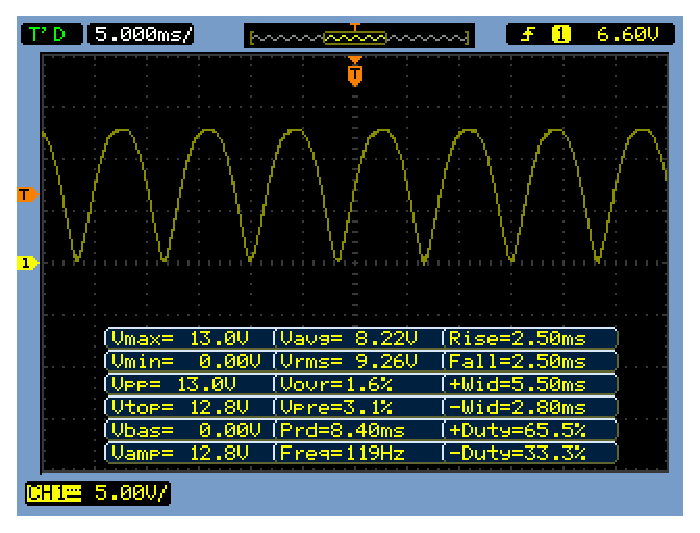
\includegraphics[scale=0.7]{Imagens/3.3.1onda_completa/3} \caption{Medida da tensão no nó 3 \label{fig:q2-no3}}
\par\end{centering}
\end{figure}



\begin{figure}[h!]
\begin{centering}
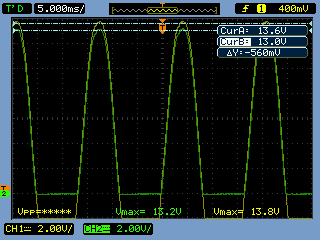
\includegraphics[scale=0.7]{Imagens/3.3.1onda_completa/31} \caption{Medida da tensão diferencial entre os nós 2 e 3 \label{fig:Fig-45}}
\par\end{centering}
\end{figure}


\begin{figure}[h!]
\begin{centering}
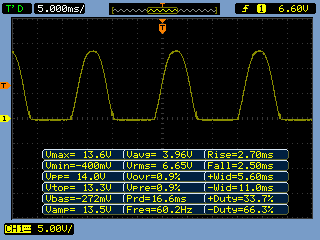
\includegraphics[scale=0.7]{Imagens/3.3.1onda_completa/no1} \caption{Medida da tensão no nó 1 \label{fig:q2-no1}}
\par\end{centering}
\end{figure}

\newpage

\begin{figure}[h!]
\begin{centering}
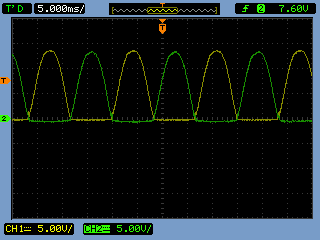
\includegraphics[scale=0.7]{Imagens/3.3.1onda_completa/no12} \caption{Medida da tensão nos nós 1 e 2 \label{fig:Fig-45}}
\par\end{centering}
\end{figure}


\begin{figure}[h!]
\begin{centering}
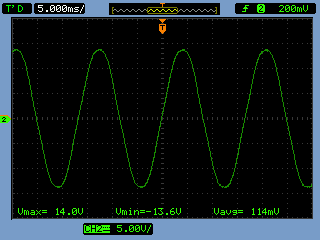
\includegraphics[scale=0.7]{Imagens/3.3.1onda_completa/p1q3} \caption{Medida da tensão diferencial entre os nós 2 e 3 \label{fig:Fig-45}}
\par\end{centering}
\end{figure}



\newpage

\begin{figure}[h!]
\begin{centering}
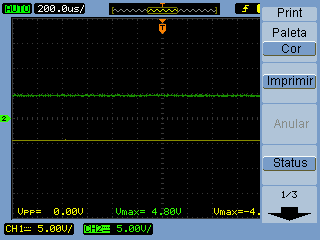
\includegraphics[scale=0.7]{Imagens/3.4duplicador_tensao/423} \caption{Medida da tensão diferencial entre os nós 2 e 3 \label{fig:Fig-45}}
\par\end{centering}
\end{figure}


\newpage
\begin{figure}[h!]
\begin{centering}
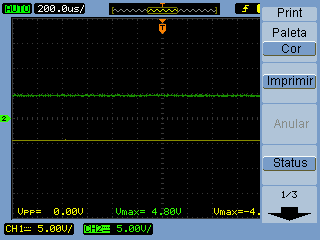
\includegraphics[scale=0.7]{Imagens/3.4duplicador_tensao/423} \caption{Tensão de saída nos nós 1 e 2 \label{fig:q4-no12}}
\par\end{centering}
\end{figure}


\begin{figure}[h!]
\begin{centering}
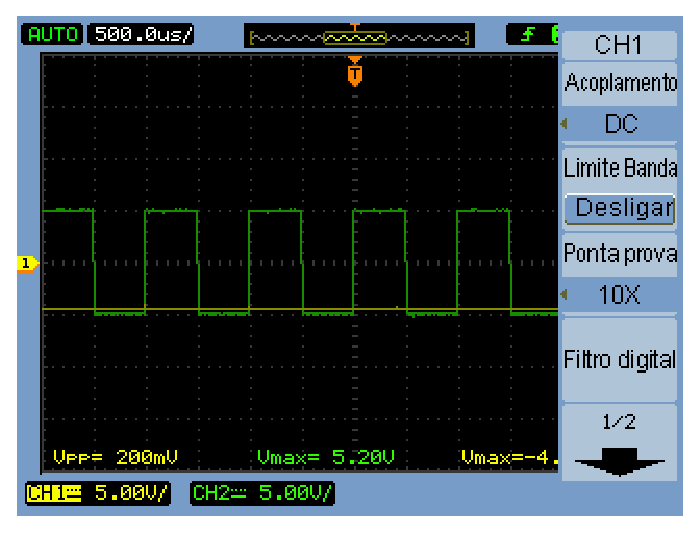
\includegraphics[scale=0.7]{Imagens/3.4duplicador_tensao/444} \caption{Análise do sinal de saída no nó x \label{fig:q4-no}}
\par\end{centering}
\end{figure}


\begin{figure}[h!]
\begin{centering}
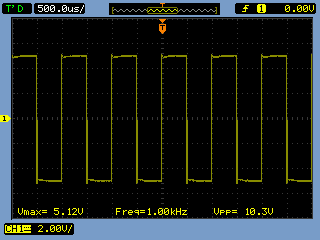
\includegraphics[scale=0.7]{Imagens/3.4duplicador_tensao/Vin} \caption{Onda de entrada do circuito\label{fig:q4-vin}}
\par\end{centering}
\end{figure}



\begin{figure}[h!]
\begin{centering}
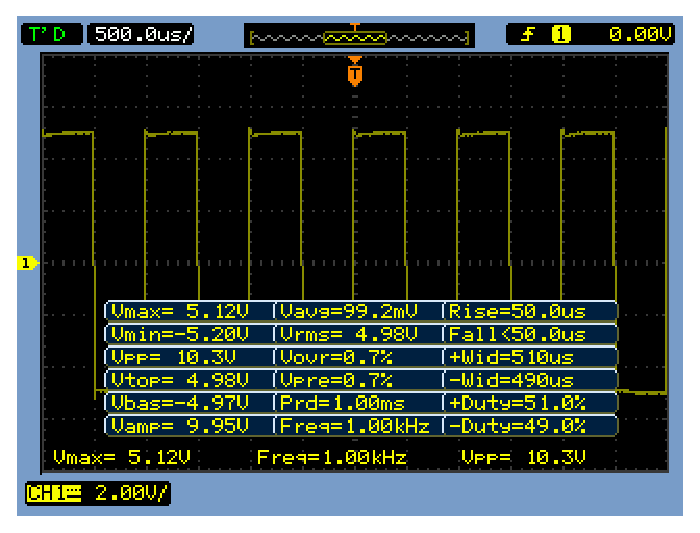
\includegraphics[scale=0.7]{Imagens/3.4duplicador_tensao/Vinmedidas} \caption{Medidas da onda de entrada do circuito \label{fig:q4-vindata}}
\par\end{centering}
\end{figure}


\newpage
\begin{figure}[h!]
\begin{centering}
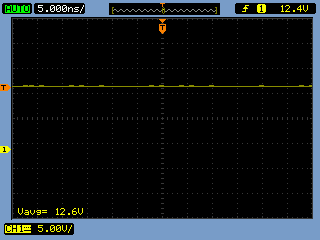
\includegraphics[scale=0.7]{Imagens/3.3.4capacitor_paralelo/3cao1} \caption{Característica onda após a inserção de capacitor em paralelo \label{fig:Fig-45}}
\par\end{centering}
\end{figure}




\end{document}
